\documentclass[a4paper,12pt]{article}
\usepackage[brazil, english]{babel}
\usepackage[utf8]{inputenc}
\usepackage[T1]{fontenc}
\usepackage{geometry}
\usepackage{setspace}
\usepackage{titlesec}
\usepackage{hyperref}
\usepackage{graphicx}
\usepackage{caption}
\usepackage{subcaption}
\usepackage{fancyhdr}
\setlength{\headheight}{15pt}
\addtolength{\topmargin}{-2.5pt}
\usepackage{xcolor}
\usepackage{amsmath, amssymb, bm}
\usepackage{mathtools}
\usepackage{cancel}
\usepackage{tikz}
\usepackage{newunicodechar}
\usepackage{ragged2e}
\usepackage{setspace}
\usepackage{tikz-3dplot} % Necessário para coordenadas 3D
\usetikzlibrary{intersections}
\usepackage{siunitx}
\usetikzlibrary{3d, arrows.meta}
\usepackage{booktabs}


\usepackage{color}
\definecolor{myblue}{rgb}{.8, .8, 1}

\definecolor{ao(english)}{rgb}{0.0, 0.5, 0.0}

\usepackage{amsmath}
\usepackage{empheq}

\newlength\mytemplen
\newsavebox\mytempbox

\makeatletter
\newcommand\mybluebox{%
    \@ifnextchar[%]
       {\@mybluebox}%
       {\@mybluebox[0pt]}}

\def\@mybluebox[#1]{%
    \@ifnextchar[%]
       {\@@mybluebox[#1]}%
       {\@@mybluebox[#1][0pt]}}

\def\@@mybluebox[#1][#2]#3{
    \sbox\mytempbox{#3}%
    \mytemplen\ht\mytempbox
    \advance\mytemplen #1\relax
    \ht\mytempbox\mytemplen
    \mytemplen\dp\mytempbox
    \advance\mytemplen #2\relax
    \dp\mytempbox\mytemplen
    \colorbox{myblue}{\hspace{1em}\usebox{\mytempbox}\hspace{1em}}}
\makeatother

\usepackage[most]{tcolorbox}

\newtcbox{\mymath}[1][]{%
    nobeforeafter, math upper, tcbox raise base,
    enhanced, colframe=blue!30!black,
    colback=blue!30, boxrule=1pt,
    #1}

\tcbset{
    highlight math style={
        enhanced,
        colframe=red!60!black,
        colback=yellow!50,
        arc=4pt,
        boxrule=1pt,
        drop fuzzy shadow
    }
    }

\usepackage{physics}
\usepackage{pgfplots}
\pgfplotsset{compat=1.17}

\linespread{1.5}

\definecolor{ao(english)}{rgb}{0.0, 0.5, 0.0}
\definecolor{byzantium}{rgb}{0.44, 0.16, 0.39}
\newunicodechar{∘}{\circ}

%%%%%%%%%%%%%%%%%%%%%%%%%%%%%%%%%%%%%%%%%%%%%%%%%%
% These are some new commands that may be useful 
% for paper writing in general. If other new commands
% are needed for your specific paper, please feel 
% free to add here. 
%
% The currently available commands are organized in: 
% 1) Systems
% 2) Quantities
% 3) Energies and units
% 4) particle species
% 5) Colors package
% 6) hyperlink
%%%%%%%%%%%%%%%%%%%%%%%%%%%%%%%%%%%%%%%%%%%%%%%%%%

\usepackage{amsmath}
\usepackage{amssymb}
\usepackage{upgreek}
\usepackage{multirow}
\usepackage{setspace}% http://ctan.org/pkg/setspace
\usepackage{fancyhdr}
\usepackage{datetime}

% 1) SYSTEMS
\newcommand{\btc}               {\textbf{BTC}}
\newcommand{\btcspace}          {\textbf{BTC} }
\newcommand{\pow}               {\textbf{PoW}}

% 4) definition to references, biblatex and hyperlink
\usepackage[backend=bibtex, 
style=nature,  %style reference.
sorting=none,
firstinits=true %first name abbreviate
]{biblatex}

\usepackage{hyperref}
\hypersetup{
    colorlinks=true, %set "true" if you want colored links
    linktoc=all,     %set to "all" if you want both sections and subsections linked
    linkcolor=blue,  %choose some color if you want links to stand out
    citecolor= blue, % color of \cite{} in the text.
    urlcolor  = blue, % color of the link for the paper in references.
}

% 5) Tikz and figures
\usepackage{epsfig}
\usepackage{lmodern}
\usepackage{mathtools}
\usepackage[utf8]{luainputenc}
\usepackage{xspace}
\usepackage{tikz}
\usepackage{pgfplots}
\pgfplotsset{compat=newest}

\usetikzlibrary{positioning}
\usepackage{subcaption}

% 6) colors:
\usepackage{xcolor}
\definecolor{ao(english)}{rgb}{0.0, 0.5, 0.0} % dark green

% 7) Add lines numbers
%\usepackage{lineno}

% add pdf file to thesis:
\usepackage{pdfpages}

\hypersetup{
    colorlinks=true,% make the links colored
    linkcolor=blue
}

\usepackage{setspace}
\addbibresource{bibliography.bib}

\newcommand{\printingbibliography}{%

    \pagestyle{myheadings}
    \markright{}
    \sloppy
    \printbibliography[heading=bibintoc, % add to table of contents
                   title=Refer\^encias % Chapter name
                  ]
    \fussy%
}
\PassOptionsToPackage{table}{xcolor}

\pagestyle{fancy}
\fancyhf{}
\renewcommand{\headrulewidth}{0pt}
\fancyhead[R]{\thepage}

\geometry{a4paper,top=30mm,bottom=20mm,left=30mm,right=20mm}

\titleformat*{\section}{\bfseries\large}
\titleformat*{\subsection}{\bfseries\normalsize}

\title{Concurso Público do Instituto Federal \\ Banco de Questões e Respostas \\ Professor do EBTT \textbf{\large F\'isica}.}
\author{Andr\'e V. Silva \\ \texttt{\url{www.andrevsilva.com}}}
\date{\today}

\begin{document}

\maketitle

\justifying

\noindent\rule{\linewidth}{0.6pt}\\

\begin{flushleft}
\textbf{\textcolor{blue}{\Large Q30 - IFC 2023 - As leis da Termodinâmica.}}\\
\noindent
-- O gráfico abaixo apresenta um \colorbox{red!20}{ciclo refrigerador em um diagrama \( P \times V \):}

\begin{center}
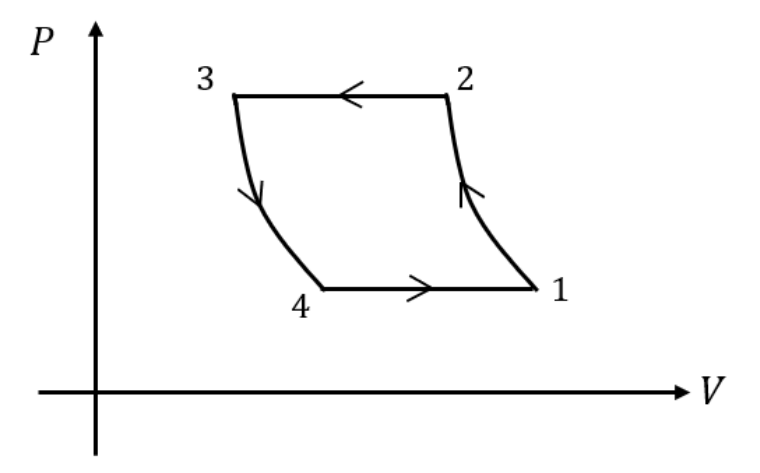
\includegraphics[width=0.6\textwidth]{figures/ciclo_refrigerador.png}
\end{center}

Os pontos \(1\), \(2\), \(3\) e \(4\) representam quatro estados para o fluido refrigerante utilizado no ciclo.  
. O aparelho refrigerador é composto por um compressor, um radiador externo, uma válvula de expansão e uma serpentina interna.  
Enquanto os \colorbox{green!20}{processos \(1 \to 2\) e \(3 \to 4\) são adiabáticos}, \colorbox{blue!20}{os processos \(2 \to 3\) e \(4 \to 1\)} \colorbox{blue!20}{são isobáricos}.  O aparelho refrigerador é composto por um compressor, um radiador externo, uma válvula de expansão e uma serpentina interna.  

Sendo assim, analise as assertivas abaixo, assinalando \(V\), se verdadeiras, ou \(F\), se falsas.

\begin{itemize}
    \item[(\ )] A etapa \(1 \to 2\) do ciclo ocorre no compressor.
    \item[(\ )] O estado indicado pelo ponto \(2\) é onde o fluido se encontra na maior temperatura durante o ciclo.
    \item[(\ )] O estado indicado pelo ponto \(4\) é onde o fluido se encontra na menor temperatura durante o ciclo.
    \item[(\ )] O fluido refrigerante se vaporiza ao passar pela válvula de expansão, absorvendo grandes quantidades de energia na forma de calor do seu entorno.
\end{itemize}

A ordem correta de preenchimento dos parênteses, de cima para baixo, é: \underline{\hspace{3cm}}

\begin{itemize}
\item[(A)] V - V - V - V.
\item[(B)] F - F - F - F.
\item[(C)] F - V - F - F.
\item[(D)] F - F - V - V.
\item[(E)] V - V - F - F.
\end{itemize}

\vspace{0.5cm}

\textcolor{red}{\textbf{Solução:}}\\

\subsection*{Introdução e teoria}

Um \textbf{ciclo de refrigeração} ideal é um processo termodinâmico cíclico, no qual um fluido refrigerante realiza trocas de calor com duas fontes térmicas: uma fria (interior da geladeira) e uma quente (ambiente).  

O ciclo típico é formado pelas seguintes etapas:
\begin{enumerate}
    \item \textbf{Compressão adiabática (1 → 2):} o fluido gasoso é comprimido, aumentando sua pressão e temperatura. Este processo ocorre no compressor.
    \item \textbf{Rejeição de calor isobárica (2 → 3):} o fluido, agora em alta pressão e alta temperatura, libera calor para o ambiente externo, geralmente se condensando.
    \item \textbf{Expansão adiabática (3 → 4):} o fluido sofre expansão rápida (na válvula de expansão), diminuindo sua pressão e temperatura.
    \item \textbf{Absorção de calor isobárica (4 → 1):} o fluido, agora frio, percorre a serpentina interna absorvendo calor do interior do refrigerador e evaporando.
\end{enumerate}

\subsection*{Análise das alternativas}

\begin{itemize}
    \item[(1)] \textbf{A etapa \(1 \to 2\) do ciclo ocorre no compressor.}  
    Verdadeira. No compressor o fluido é comprimido, aumentando sua pressão e temperatura.  

    \item[(2)] \textbf{O estado indicado pelo ponto \(2\) é onde o fluido se encontra na maior temperatura durante o ciclo.}  
    Verdadeira. No ponto \(2\), após a compressão adiabática, a temperatura é máxima.  

    \item[(3)] \textbf{O estado indicado pelo ponto \(4\) é onde o fluido se encontra na menor temperatura durante o ciclo.}  
    Verdadeira. No ponto \(4\), após a expansão adiabática, a temperatura é mínima.  

    \item[(4)] \textbf{O fluido refrigerante se vaporiza ao passar pela válvula de expansão, absorvendo grandes quantidades de energia na forma de calor do seu entorno.}  
    Verdadeira. Após a válvula de expansão o fluido já sai em baixa temperatura e parcialmente vapor, completando a vaporização na serpentina interna ao absorver calor do ambiente refrigerado. A interpretação da frase está correta considerando o processo imediatamente após a válvula.
\end{itemize}

\subsection*{Resposta final}

A sequência correta de preenchimento dos parênteses, de cima para baixo, é:
\[
\boxed{V \quad V \quad V \quad V}
\]

A resposta correta é alternativa \colorbox{green!50}{\textbf{A}}.
\end{flushleft}

\noindent\rule{\linewidth}{0.6pt}\\

\section*{Introdução ao Ciclo Stirling Ideal}

O \colorbox{yellow!30}{\textbf{ciclo Stirling ideal} é um dos ciclos termodinâmicos mais conhecidos e estudados}, utilizado como modelo para motores e refrigeradores de alta eficiência. Esse ciclo foi proposto por Robert Stirling em 1816 como uma alternativa mais eficiente e segura aos motores a vapor da época.

Trata-se de um \colorbox{green!30}{\textit{ciclo termodinâmico fechado}, no qual um gás ideal passa por quatro} \colorbox{green!30}{transformações reversíveis}, sendo duas isotérmicas e duas isocóricas (ou isovolumétricas), realizadas em sequência e formando um ciclo no diagrama \(p\)-\(V\).

O ciclo Stirling ideal é composto pelas seguintes etapas:

\begin{enumerate}
    \item \colorbox{green!30}{\textbf{Expansão isotérmica (\(A \to B\))}}: o gás se expande a temperatura constante, absorvendo calor de uma fonte quente enquanto realiza trabalho.
    \item \colorbox{green!30}{\textbf{Resfriamento isocórico (\(B \to C\))}}: o volume permanece constante, e o gás libera calor, diminuindo sua pressão e temperatura.
    \item \colorbox{green!30}{\textbf{Compressão isotérmica (\(C \to D\))}}: o gás é comprimido a temperatura constante, cedendo calor para uma fonte fria enquanto recebe trabalho.
    \item \colorbox{green!30}{\textbf{Aquecimento isocórico (\(D \to A\))}}: o volume permanece constante, e o gás absorve calor, aumentando sua pressão e temperatura, retornando ao estado inicial.
\end{enumerate}

O \colorbox{green!30}{ciclo Stirling apresenta eficiência teórica igual à do ciclo de Carnot}, quando operado entre as mesmas temperaturas extremas, pois também é formado por transformações reversíveis. Seu diferencial prático está no uso de regeneradores de calor para melhorar a eficiência, armazenando calor durante as etapas isocóricas.

\bigskip

Essas características tornam o ciclo Stirling um importante objeto de estudo para o desenvolvimento de motores alternativos e sistemas de refrigeração com menor impacto ambiental e alta eficiência energética.


\begin{flushleft}
\textbf{\textcolor{blue}{\Large Q51 - IFC 2023 - As leis da Termodinâmica.}}\\
\noindent
\textbf{Ciclos termodinâmicos são processos} em que se deseja que o sistema realize trabalho ou que certo trabalho seja realizado sobre o sistema. Os ciclos termodinâmicos podem ser dos mais variados tipos. O ciclo Stirling ideal, representado no gráfico abaixo, é um dos mais conhecidos.

\begin{center}
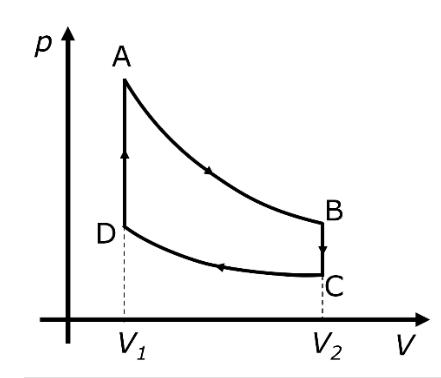
\includegraphics[width=0.5\textwidth]{figures/ciclo_stirling.png}
\end{center}

Com base no exposto acima, relacione a Coluna 1 à Coluna 2.

\textbf{Coluna 1}

\begin{enumerate}
    \item Curva \( A \to B \)
    \item Curva \( B \to C \)
    \item Curva \( C \to D \)
    \item Curva \( D \to A \)
\end{enumerate}

\textbf{Coluna 2}

\begin{enumerate}
    \item[(\ )] Isocórica
    \item[(\ )] Isotérmica
    \item[(\ )] Recebe calor
    \item[(\ )] Realiza trabalho
\end{enumerate}

A ordem correta de preenchimento dos parênteses, de cima para baixo, é:

\begin{itemize}
\item[(A)] 1 -- 2 -- 3 -- 4
\item[(B)] 2 -- 1 -- 4 -- 3
\item[(C)] 2 -- 3 -- 4 -- 1
\item[(D)] 4 -- 3 -- 1 -- 2
\item[(E)] 4 -- 1 -- 3 -- 2
\end{itemize}

\vspace{0.5cm}

\textcolor{red}{\textbf{Solução:}}\\

\section*{Resolução}

Para resolver a questão, analisamos cada uma das curvas do ciclo Stirling ideal representado no gráfico \(p\)-\(V\). O ciclo é formado por duas transformações isotérmicas e duas isocóricas, em sequência.

\bigskip

\textbf{Etapa por etapa:}

\begin{itemize}
    \item \textbf{Curva \( A \to B \)}: 
    Nesta etapa, o volume aumenta (\(V_1 \to V_2\)) e a curva é hiperbólica, típica de um processo isotérmico. Assim, é uma \textbf{transformação isotérmica} na qual o sistema \textbf{recebe calor e realiza trabalho}.
    
    \item \textbf{Curva \( B \to C \)}:
    Aqui, o volume permanece constante (\(V_2\)) e a pressão diminui, caracterizando uma \textbf{transformação isocórica}. Não há trabalho realizado (pois o volume não varia), mas o sistema libera calor.
    
    \item \textbf{Curva \( C \to D \)}:
    Nessa etapa, o volume diminui (\(V_2 \to V_1\)) com uma curva hiperbólica, ou seja, outra \textbf{transformação isotérmica}. O sistema realiza trabalho negativo (sofre trabalho) e cede calor.
    
    \item \textbf{Curva \( D \to A \)}:
    Por fim, o volume permanece constante (\(V_1\)) e a pressão aumenta, configurando outra \textbf{transformação isocórica}, na qual o sistema absorve calor.
\end{itemize}

\bigskip

\textbf{Correspondências:}

\begin{itemize}
    \item Isocórica: curva \( B \to C \) (item 2)
    \item Isotérmica: curva \( A \to B \) (item 1)
    \item Recebe calor: curva \( D \to A \) (item 4)
    \item Realiza trabalho: curva \( C \to D \) (item 3)
\end{itemize}

Assim, a ordem correta dos itens, de cima para baixo, é:
\[
\boxed{2 \ -- \ 1 \ -- \ 4 \ -- \ 3}
\]

\bigskip

A resposta correta é alternativa \colorbox{green!50}{\textbf{C}}.
\end{flushleft}

\noindent\rule{\linewidth}{0.6pt}\\

\begin{flushleft}
\textbf{\textcolor{blue}{\Large Q30 - IFC 2023 - As leis da Termodinâmica.}}\\
\noindent

\begin{itemize}
\item[(A)] 
\item[(B)] 
\item[(C)] 
\item[(D)] 
\item[(E)] 
\end{itemize}

\vspace{0.5cm}

\textcolor{red}{\textbf{Solução:}}\\


A resposta correta é alternativa \colorbox{green!50}{\textbf{...}}.
\end{flushleft}

\noindent\rule{\linewidth}{0.6pt}\\


%%%%%%%% Bibliography 
% Os comandos para incluir as referências bibliográficas
%\printingbibliography

\end{document}
